% mnras_template.tex 
%
% LaTeX template for creating an MNRAS paper
%
% v3.0 released 14 May 2015
% (version numbers match those of mnras.cls)
%
% Copyright (C) Royal Astronomical Society 2015
% Authors:
% Keith T. Smith (Royal Astronomical Society)

% Change log
%
% v3.0 May 2015
%    Renamed to match the new package name
%    Version number matches mnras.cls
%    A few minor tweaks to wording
% v1.0 September 2013
%    Beta testing only - never publicly released
%    First version: a simple (ish) template for creating an MNRAS paper

%%%%%%%%%%%%%%%%%%%%%%%%%%%%%%%%%%%%%%%%%%%%%%%%%%
% Basic setup. Most papers should leave these options alone.
\documentclass[fleqn,usenatbib]{mnras}

% MNRAS is set in Times font. If you don't have this installed (most LaTeX
% installations will be fine) or prefer the old Computer Modern fonts, comment
% out the following line
\usepackage{newtxtext,newtxmath}
% Depending on your LaTeX fonts installation, you might get better results with one of these:
%\usepackage{mathptmx}
%\usepackage{txfonts}

% Use vector fonts, so it zooms properly in on-screen viewing software
% Don't change these lines unless you know what you are doing
\usepackage[T1]{fontenc}

% Allow "Thomas van Noord" and "Simon de Laguarde" and alike to be sorted by "N" and "L" etc. in the bibliography.
% Write the name in the bibliography as "\VAN{Noord}{Van}{van} Noord, Thomas"
\DeclareRobustCommand{\VAN}[3]{#2}
\let\VANthebibliography\thebibliography
\def\thebibliography{\DeclareRobustCommand{\VAN}[3]{##3}\VANthebibliography}


%%%%% AUTHORS - PLACE YOUR OWN PACKAGES HERE %%%%%

% Only include extra packages if you really need them. Common packages are:
\usepackage{graphicx}	% Including figure files
\usepackage{amsmath}	% Advanced maths commands
\usepackage{amssymb}	% Extra maths symbols

%%%%%%%%%%%%%%%%%%%%%%%%%%%%%%%%%%%%%%%%%%%%%%%%%%

%%%%% AUTHORS - PLACE YOUR OWN COMMANDS HERE %%%%%

% Please keep new commands to a minimum, and use \newcommand not \def to avoid
% overwriting existing commands. Example:
%\newcommand{\pcm}{\,cm$^{-2}$}	% per cm-squared

%%%%%%%%%%%%%%%%%%%%%%%%%%%%%%%%%%%%%%%%%%%%%%%%%%

%%%%%%%%%%%%%%%%%%% TITLE PAGE %%%%%%%%%%%%%%%%%%%

% Title of the paper, and the short title which is used in the headers.
% Keep the title short and informative.
\title[ASPIRED]{Automate your spectral data reduction with Automated SpectroPhotometric Image REDuction (ASPIRED) pipeline builder}

% The list of authors, and the short list which is used in the headers.
% If you need two or more lines of authors, add an extra line using \newauthor
\author[M. C. Lam et al.]{
Marco C. Lam,$^{1, 2, 3}$\thanks{E-mail: lam@tau.ac.il}
Robert J. Smith,$^{2}$
Josh Veitch-Michaelis,$^{2}$
P. Ross McWhirter,$^{2}$
Iain A. Steele,$^{2}$
\newauthor
Iair Arcavi,$^{1}$
Lukasz Wyrzykowski$^{3}$
\\
% List of institutions
$^{1}$Tel Aviv University\\
$^{2}$Liverpool John Moores University\\
$^{3}$Warsaw University
}

% These dates will be filled out by the publisher
\date{Accepted XXX. Received YYY; in original form ZZZ}

% Enter the current year, for the copyright statements etc.
\pubyear{2021}

% Don't change these lines
\begin{document}
\label{firstpage}
\pagerange{\pageref{firstpage}--\pageref{lastpage}}
\maketitle

% Abstract of the paper
\begin{abstract}
We provide a suite of publicly available spectral data reduction software
to facilitate rapid scientific outcomes from time-domain observations. The Automated
SpectroPhotometric REDuction (\textsc{ASPIRED}) pipeline builder, designed for common
use on different instruments. The default settings support many typical long-slit
spectrometer configurations, whilst it also offers a flexible set of functions for
users to refine and tailor-make their automated pipelines to an instrument's
individual characteristics. Such automation provides near real-time data reduction
to allow adaptive observing strategies, which is particularly important in the Time
Domain Astronomy.
\end{abstract}

% Select between one and six entries from the list of approved keywords.
% Don't make up new ones.
\begin{keywords}
keyword1 -- keyword2 -- keyword3
\end{keywords}

%%%%%%%%%%%%%%%%%%%%%%%%%%%%%%%%%%%%%%%%%%%%%%%%%%

%%%%%%%%%%%%%%%%% BODY OF PAPER %%%%%%%%%%%%%%%%%%

\section{Introduction}
With major global investments in multi-wavelength and multi-messenger surveys, time domain
astronomy is entering a golden age. To maximally scientific exploit discoveries from these
facilities rapid spectroscopic follow-up observations of transient objects~(e.g.,\ supernovae,
gravitational wave optical counterparts etc.) will provide crucial {\em astrophysical} 
interpretations. Part of the OPTICON\footnote{\url{https://www.astro-opticon.org}} project
coordinates the operation of a network of largely self-funded European robotic and conventional
telescopes, coordinating common science goals and providing the tools to deliver science-ready
photometric and spectroscopic data. As part of this activity SPRAT~\citep{2014SPIE.9147E..8HP}
was developed as a compact, reliable, low-cost and high-throughput spectrograph and appropriate
for deployment on a wide range of 1-4\,m class telescopes. Installed on the Liverpool Telescope
since 2014, the deployable slit and grating mechanism and optical fibre based calibration
system make the instrument self-contained. Copies of SPRAT are being built for other 
telescopes. Our final task is to deliver software that can be easily configured to build
pipelines for long slit spectrographs on different telescopes.

The ``industrial standard'' of spectral and image reduction is of no doubt the
\textsc{iraf} software~\citep{1986SPIE..627..733T, 1993ASPC...52..173T}. It has powered many
reduction engines in the past and present. However, unfortunately, the software has reached
the end-of-support state where there will no longer be any official support to the software
and it relies entirely on community support\footnote{\url{https://iraf-community.github.io}}.
In this generation of user-side Astronomy data handling and processing, as well as the
computing courses for Scientists, \textsc{Python} is among the most popular languages due to
its ease to use with a shallow learning curve, readable syntax and simple way to ``glue''
different pieces of software together. Its flexibility to serve as a scripting and an
object-oriented language makes it useful in many use cases: demonstrating with visual tools
with little overhead, prototyping, web-serving, be compiled if wanted. This broad range of
functionality and high level usage make it relatively inefficient. However, \textsc{Python}
is an excellent choice of language to build wrappers over highly efficient and well
established codes. In fact, some of the most used packages,
\textsc{scipy}~\citep{2020SciPy-NMeth} and \textsc{numpy}~\citep{2020NumPy-Array},
are written in \textsc{Fortran} and \textsc{C} respectively. Multi-threading and -processing
are also possible with built-in and other third party packages, e.g.\ mpi4py~\citep{DALCIN20111124}. 
Varies efforts are made to develop a software for the (this/)next-generation data reduction,
for example, \textsc{PypeIt}~\citep{pypeit:zenodo, pypeit:joss_pub} for taylor-made reductions
for a list of instruments, \textsc{PyReduce}~\citep{2021A&A...646A..32P} designed for optimal
Echelle spectral reduction which does not handle sky subtraction;
in the \textsc{Astropy} ``Universe''~\citep{astropy:2013, astropy:2018}, \textsc{specreduce}
is likely to be the next-generation user-focused data reduction package, but it is far from
the stage of deployment at the time of writing, \textsc{pyDIS} which has all the essential
ingredients for reducing spectra but it is out of maintenance since 2016, \textsc{specutils}
handles spectral analysis and manipulation but not the reduction itself.

We use SPRAT-family as our first-light instruments for the development, but our aim is to
allow high level tools for users to build and fine tune their pipelines to support
a wide range of instruments~\citep{2020arXiv201203505L, marco_2021_4463569}. As of time of
writing, we have successfully reduced data from the William Herschel Telescope
\textit{Intermediate-dispersion Spectrograph and Imaging System}
\footnote{\url{https://www.ing.iac.es/astronomy/instruments/isis}}~(WHT/ISIS), Las Cumbres
Observatory FLOYDS~\citep[LCO/FLOYDS]{2013PASP..125.1031B}, Gemini Observatory
\textit{Gemini Multi-Object Spectrographs} long slit
mode~\citep[Gemini/GMOS-LS]{2004PASP..116..425H}, Gran Telescopio Canarias \textit{Optical
System for Imaging and low-Intermediate-Resolution Integrated
Spectroscopy}~\citep[GTC/OSIRIS]{2000SPIE.4008..623C}, and Telescopio Nazionale Galileo
\textit{Device Optimized for the LOw
RESolution\footnote{\url{http://www.tng.iac.es/instruments/lrs}}}~(TNG/DOLORES); all of
these are unofficial pipelines.

By delivering near real-time data reduction we will facilitate automated or interactive
decision making, allowing "on-the-fly" modification of observing strategies and rapid
triggering of other facilities.

This paper is organised as follow, in section 2.

\section{Development and Structure of ASPIRED}
The development of ASPIRED is coordinated on Github\footnote{\url{https://github.com/cylammarco/ASPIRED}}, which provides version control using \textsc{git}\footnote{\url{https://git-scm.com}}, issue and bug tracking, high-level project management, automation with \textsc{Github Actions} upon each \texttt{commit} for:

\begin{enumerate}
    \item Continuous Integration~(CI) to install the software in \textsc{Linux}, \textsc{Mac} and \textsc{Windows} system, and then perform unit tests with \textsc{pytest}~\citep{pytest6.2},
    \item generating test coverage report with \textsc{Coveralls}\footnote{\url{https://coveralls.io/github/cylammarco/ASPIRED}} which identifies lines in thee script that are missed from the tests,
    \item Continuous Deployment~(CD) through \textsc{PyPI}\footnote{\url{https://pypi.org/project/aspired}} that allows immediate availability of the latest numbered version,
    \item dependency version tracking with \textsc{Dependabot}\footnote{\url{https://dependabot.com}}, and
    \item generating API documentation powered by \textsc{Sphinx}\footnote{\url{https://www.sphinx-doc.org/en/master}} hosted on Read the Docs\footnote{\url{https://aspired.readthedocs.io/en/latest}}.
\end{enumerate}

The development goal of ASPIRED was to design a software that is as modular and
portable as possible, we are still maintaining the principal. We rely on as few
external dependencies as possible, the ones we use are those requiring substantial
programming effort and have a proven track record on the reliability and/or
with a plan to keep up with the maintenance  in the foreseeable future. The top
level explicit dependencies are --
\textsc{astroscrappy}~\citep{curtis_mccully_2018_1482019, 2001PASP..113.1420V}
\textsc{astopy}~\citep{astropy:2013, astropy:2018},
\textsc{ccdproc}~\citep{matt_craig_2017_1069648},
\textsc{numpy}~\citep{2020NumPy-Array}
\textsc{plotly}~\citep{plotly},
\textsc{scipy}~\citep{2020SciPy-NMeth}
\textsc{spectres}~\citep{2017arXiv170505165C}, and
\textsc{statsmodels}~\citep{seabold2010statsmodels}. 

This article is not intended to serve as an API document, nor is it to review
various methods concerning spectral extraction. Only the high-level
descriptions and the Scientific and Mathematical technicalities that are
important to the data reduction processes are reported here. The initial
work package divided the project broadly into 3 highest level independent
components:

\subsection*{graphical user interface (not in active development)}
In the beginning, we commissioned a prototyping of the graphical user
interface\footnote{\url{https://github.com/cylammarco/gASPIRED}}
\textsc{Electron}\footnote{\url{https://www.electronjs.org}}, which wraps on top of
\textsc{ASPIRED} without needing to adapt the code to allow the interaction, this is
possible for a few reasons: first, \textsc{Python} is an interpreter, it can execute
in run time. It is very easy to run itself as a server to handle the response from 
\textsc{Electron}; second, the using of
\textsc{plotly}\footnote{\url{https://plotly.com}} as the plotting
library can enable interactive plotting easily; exporting static and dynamic plots
can be done with ease; third, there is a \textsc{JavaScript} version of
\textsc{SAOImageDS9}\footnote{\url{https://sites.google.com/cfa.harvard.edu/saoimageds9}}
that allows rapid and easy interactive image manipulation in a familiar
fashion~\citep{eric_mandel_2021_596052}. Given the way how \textsc{Electron} and
\textsc{JS9} work like a web-service, this prototype also shows that this can also
be deployed as an online tool. This is, however, no longer in active development
and is only served as a technology demonstrator of its capability.

\subsection*{wavelength calibration (not part of this work)}
The wavelength calibration module is powered by
\textsc{RASCAL}~\citep{2020zndo...4117517V, 2020ASPC..527..627V}, a software
developed in conjunction but independently of \textsc{ASPIRED}. It is improved
upon the work by \citet{2018ApOpt..57.6876S}, which searches only for
\textit{plausible} sets of lines that follow good linear approximations to the
system. \textsc{RASCAL} considers the top $N$ sets simultaneously. For each
peak, the most common best-fit atlas line are chosen from the top candidate
sets. This acts like a piece-wise linear fit and allows us to extract most of
the correct matches from both the red and blue ends of the spectrum. RANdom
SAmple Consensus~\citep[RANSAC][]{fischler_bolles_1981} is used to robustly
fit a higher order polynomial model to the candidate correspondences. All what
a user is required to do is to supply a list of calibration lines~(pixels), a
list of peaks~(wavelengths), and some knowledge of the system to initialise a
most appropriate and efficient calibrator~(e.g.\ dispersion resolution).

\subsection*{the rest of the spectral extraction and calibrations (this work)}
This is the core of the \textsc{ASPIRED}, which mainly handles the spectral
extraction and calibration processes. The software is organised into
3 main parts - the \texttt{image\_reduction}, \texttt{spectral\_reduction},
and \texttt{spectrum1D}. The first two are the ``overlords'' that wraps
round all the dependant classes and functions to handle all the operations.
The last one is a data structure and stores the metadata and the extracted
data. The FITS file I/O handling is also handled by the \texttt{spectrum1D}.

\subsection*{\texttt{image\_reduction}}
This work is not intended to provide high quality image reduction, it only
provides basic image reduction methods. However, this should be sufficient
for simple optical systems, which are the target audience of \textsc{ASPIRED}.
This class allows combining, subtracting and dividing of light, dark, bias
and flat frames. The FITS header of the first light frame provided will be
copied over, while the rest will be stored as a path to the file. Meta-data
regarding the image reduction are appended to the end of the FITS header.
Depending on the convention adopted, The FITS file can be exported to contain
an empty \texttt{PrimaryHDU} with the process data stored in the first
\texttt{ImageHDU} extension as recommended in the FITS Standard
document\footnote{\url{https://fits.gsfc.nasa.gov/fits_documentation.html}},
or it can be stored directly in the \texttt{PrimaryHDU} as most users tend
to opt for. Many forms of interactive and static images can be exported as
powered by \textsc{Plotly} image renderer.

\subsection*{\texttt{spectral\_reduction}}
This is a large class that covers both 1D and 2D operations. In 2D, it
provides image rectification, spectral tracing and spectral extraction.
In 1D, it can perform wavelength calibration, flux calibration, atmospheric
extinction correction. Diagnostic images can be exported at each step
of operation, including the wavelength calibration that wraps round
\textsc{RASCAL} and uses their native plotting capability. Outputs can
be in form of FITS or ascii files, e.g.\ CSV, where possible. See the next
section for the mathematical and scientific descriptions of the various
methods.

\subsection*{\texttt{spectrum1D}}
This is a data class to provide a uniform format to store the metadata
and the extracted data throughout the entire spectral extraction process.
It provides all the FITS and ascii file I/O handling functions, where all
the higher level functions wrap over on. It is intended to keep this
structure as lightweight as possible, so it does not carry any plotting
instrutions. However, data storage in observational data is almost
exclusively done with FITS file, we believe that the inclusion of the
FITS I/O can significantly improve the usability. While there are many
plotting libraries available and there is not a unified standard
as to how to create a figure.

\section{Spectral Reduction}
In the higher level terms, a spectral reduction procedures after image
reduction includes: (1) identifying the spectrum/a, (2) tracing the
spectrum/a, (3) image distortion correction, (4) extracting the
spectrum/a, (5) wavelength calibration of the science target and a
standard star, (6) computing sensitivity curve using the standard
observations, (7) flux calibration by applying the sensitivity curve,
and finally (8) atmospheric extinction correction. We omit a few
processes which we believe they should be considered as part of the
post-extraction processes or spectral analysis and manipulation.
There are many sophisticated software with good and long track records
to handle these processes post-hoc. For example: sky glow subtraction
with \textsc{Skycorr}~\citep{2014A&A...567A..25N}, and Telluric
absorption removal with
\textsc{MoleFit}~\citep{2015A&A...576A..77S, 2015A&A...576A..78K}.
The following describes the technical details of the eight steps,
we have the following convention: the spectral image is dispersed
on the detector plane such that left is blue (small pixel number)
and right is red (large pixel number).

\subsection{Spectral Identification and Tracing}
\label{sec:tracing}
Conventionally, the spectra are first identified and then traced along
the ``ridges'' in the image to obtain the traces of the spectra.
Instead, the \texttt{ap\_trace} function works by dividing the 2D
spectrum into sub-spectra, and then each part is summed along the
spectral direction before cross-correlating with the adjacent
sub-spectra, the shift and scaling of the spectrum/a along the
spectral direction can be found simultaneously. The middle of the
2D spectrum is used as the zero point of the procedure. Here is the
detailed description of the algorithm.
\begin{enumerate}
    \item
        The input 2D spectrum is divided into \texttt{nwindow}
        sub-spectra.
    \item
        Each sub-spectrum is summed along the spectral direction
        in order to improve the signal(s) of the spectrum/a along
        the spatial direction – we call this a spatial spectrum.
    \item
        Each spatial spectrum is upscale by a factor of
        \texttt{resample\_factor} to allow for sub-pixel correlation.
        This utilises the \texttt{scipy.signal.resample()} function
        to fit the spatial profile with spline.
    \item
        The i-th spatial spectrum is then cross-correlated i+1-th
        spatial spectrum. The shift and scale at where the maximum
        occurs within the tolerance limit, \texttt{tol} will be stored.
    \item
        While the spatial spectra are being cross-correlated. They
        are aligned and stacked for peak finding and Gaussian fitting.
        Peak finding is performed with
        \texttt{scipy.signal.find\_peaks()} and returned the list of
        peaks sorted by their prominence. Only centroiding has to be
        accurate at this stage, so a Gaussian function is sufficient.
        The standard deviation of the Gaussian is only served as a
        first guess of the profile when performing optimal extraction;
        it would not be used in the case of top-hat extraction.
\end{enumerate}

This procedure is illustrated in Fig.~\ref{fig:trace}. Manually
supplying trace(s) is possible with the \texttt{add\_trace}
function. This is particularly useful for faint and/or confused
sources that are beyond the capability of the automated tracing.

\begin{figure}
    \centering
    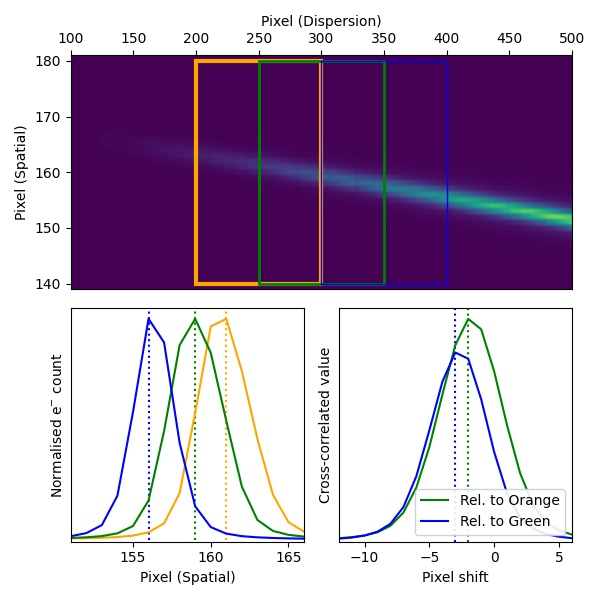
\includegraphics[width=\columnwidth]{fig_01_tracing.jpg}
    \caption{Caption}
    \label{fig:trace}
\end{figure}


\subsection{Image Rectification}
In most cases, a spectrum on the detector plane is not only tilted,
but it is also sufficiently distorted that the extraction
has to be performed along a curve. While this does not cause any
complication in the tracing, and the spatial and dispersion
directions are still notionally orthogonal to each other, these two
axes are no longer aligned with the x-y axes of the detector plane.
\textsc{PyReduce}, as aforementioned, can optimally extract this
kind of highly distorted spectra, but the lack of sky subtraction
using the ``wings'' beyond the line-spread-profile has limited the
usage in a typical single-frame extraction without an accompanying
sky~(blank) observation. Alternative to extracting along a curve,
the 2D image can be rectified based on the spectral trace and sky
emission lines before extraction to be performed on a spectrum
(nearly) perfectly aligned with the detector x-y axes.

The rectification in the spatial direction depends \textbf{only}
on the trace. Each column of pixel gets (scaled and) shifted by
resampling to align with the centre of the spectrum. This will
usually leave us with a spectrum tilted or curved in the dispersion
direction. The same procedure as to trace the spectra is applied
in the spatial direction to find the best fit polynomial solution
for shifting (and scaling) in the dispersion direction for the
last step of the rectification process.

\begin{figure}
    \centering
    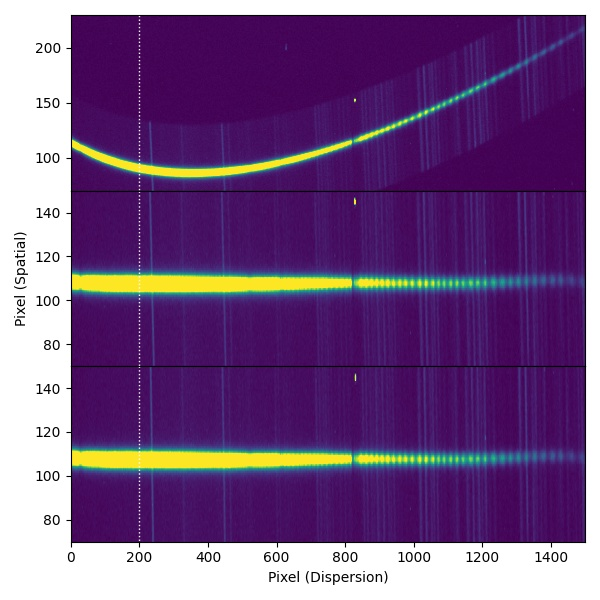
\includegraphics[width=\columnwidth]{fig_02_rectification.jpg}
    \caption{Caption}
    \label{fig:rectify}
\end{figure}

At the time of writing, this process is only possible if there is
one trace. If more than one trace is found/provided, only the first
one will get processed. The resampling is performed with
\textsc{SpectRes} which preserves the electron count. It is possible
to supply a polynomial to carry out the rectification, which would
be useful and can significantly speed up the data reduction process
of a stable optical system.

\subsection{Spectral Extraction}
\label{sec:extract}
There are a few commonly used extraction methods, some work for
all kinds of spectral images, some only work with specific
observing strategies, for example, the flat-relative optimal
extraction~\citep{2014A&A...561A..59Z}. The standard textbook
method is commonly called the tophat extraction or the normal
extraction, it simply sums the electron counts over a given
size of aperture. It is robust and easy to use. However, this
method does not deliver the maximal signal-to-noise ratio~(SNR)
from the available data. Various optimal extraction algorithms
can maximise the SNR during the process. This works by
down-weighting the wings of the spectral profile where almost
all the photons are coming from the sky but not the source. An
optimal extraction can boost the SNR, particularly for the
background-limited sources, which are the case for most
observations. The extracted spectra and their associated
uncertainties and sky background counts can be plotted for
inspection. The residual image can also be exported for
diagnostics.

\begin{figure}
    \centering
    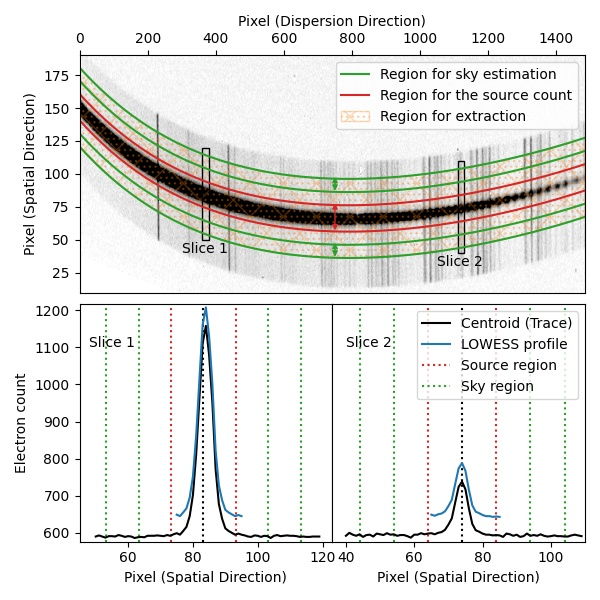
\includegraphics[width=\columnwidth]{fig_03_extraction_profile.jpg}
    \caption{Caption}
    \label{fig:extract}
\end{figure}

\subsubsection*{Tophat/Normal Extraction}
The tophat extraction does not weigh the pixels for extraction,
so every pixel has equal contribution to the source count. Thus,
it is very robust in getting the total electron count across
a slice of pixels. The sky background count can be extracted
from the regions just outside of the extraction aperture to be
subtracted from the spectrum. See Fig.~something.

\subsubsection*{Horne-86 Optimal Extraction}
\citet[hereafter H86]{1986PASP...98..609H} is the golden standard
of optimal extraction of spectrum from a modern electronic detector.
We are following the H86 recipe except for the profile modelling,
where we provide three options, the first one is a fixed Gaussian
profile, the second one uses LOcally Weighted Scatterplot
Smoothing~\citep[LOWESS]{doi:10.1080/01621459.1979.10481038}
regression to fit for a polynomial, and the last one accepts
manually supplied profile that has either the length matches the
size of the aperture or the shape of the size of the aperture by
the length of the spectrum in the dispersion direction.

The default option is to use the LOWESS fit because it is the
least sensitive to noise and cosmic ray contiminations. This is
also flexible enough to allow good fit for the profile of a
resolved galaxy. This may, however, be less accurate for
extracting a faint spectrum when the image is dominated by the
background noise. In such case, the Gaussian profile is
recommended as the profile is constructed from fitting the
line-spread-function from the total-stack of all the
subspectra~(the ones described in Sec.~\ref{sec:tracing}). If
the quality of the tracing is acceptable, the quality of the
profile should be sufficient to allow more optimal extraction
than a tophat extraction.

\subsubsection*{Marsh-89 Optimal Extraction}
\citet[hereafter M89]{1989PASP..101.1032M} improves on the H86
algorithm by fitting the change in the shape and centroid of
the profile from one end of the spectrum to the other. It is
very suited for extracted a highly tilted spectrum where the
tilting direction is aligned with either the $x$ or the $y$
axis of the detector.

The script is adapted to \textsc{Python 3} from Ian Crossfield's
set of public \textsc{Python 2} code for 
Astronomy\footnote{\url{https://people.ucsc.edu/~ianc/python/}}.

\begin{figure}
    \centering
    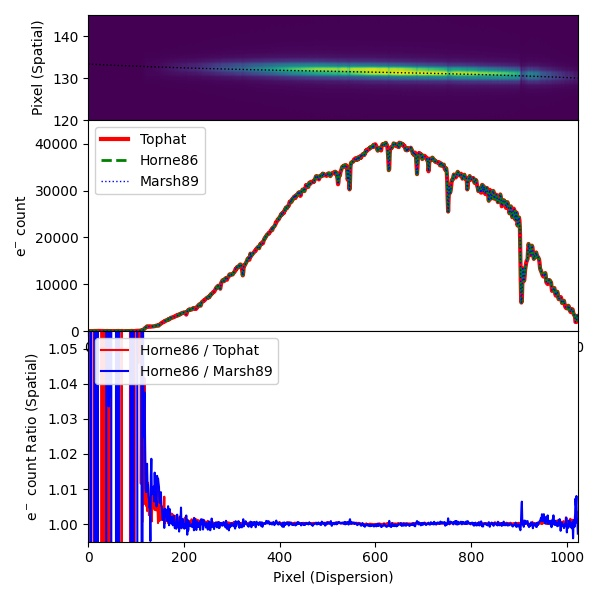
\includegraphics[width=\columnwidth]{fig_04_extraction_compared.jpg}
    \caption{Caption}
    \label{fig:extract}
\end{figure}

\subsection{Wavelength Calibration}
The wavelength calibration is powered by \textsc{RASCAL} which
is a concurrent development to this work. All the public
functions from \textsc{RASCAL} are available in \textsc{ASPIRED}
so users can have fine control over the calibration. The
diagnostic plots are the set provided by \textsc{RASCAL}.
They include the spectrum of the arc lamp at where the traces
on the science and standard frames are, which also shows where
the peaks are detected; the peak-line pairs and the constrained
space where the Hough-pairs are
selected~(see \citealt{2020ASPC..527..627V}); and a plot showing
the fitting solution and its quality.

The polynomial coefficients for the calibration can be supplied
directly, which would be useful for stable instruments that
the shift in the dispersion direction is negligible.

\begin{figure}
    \centering
    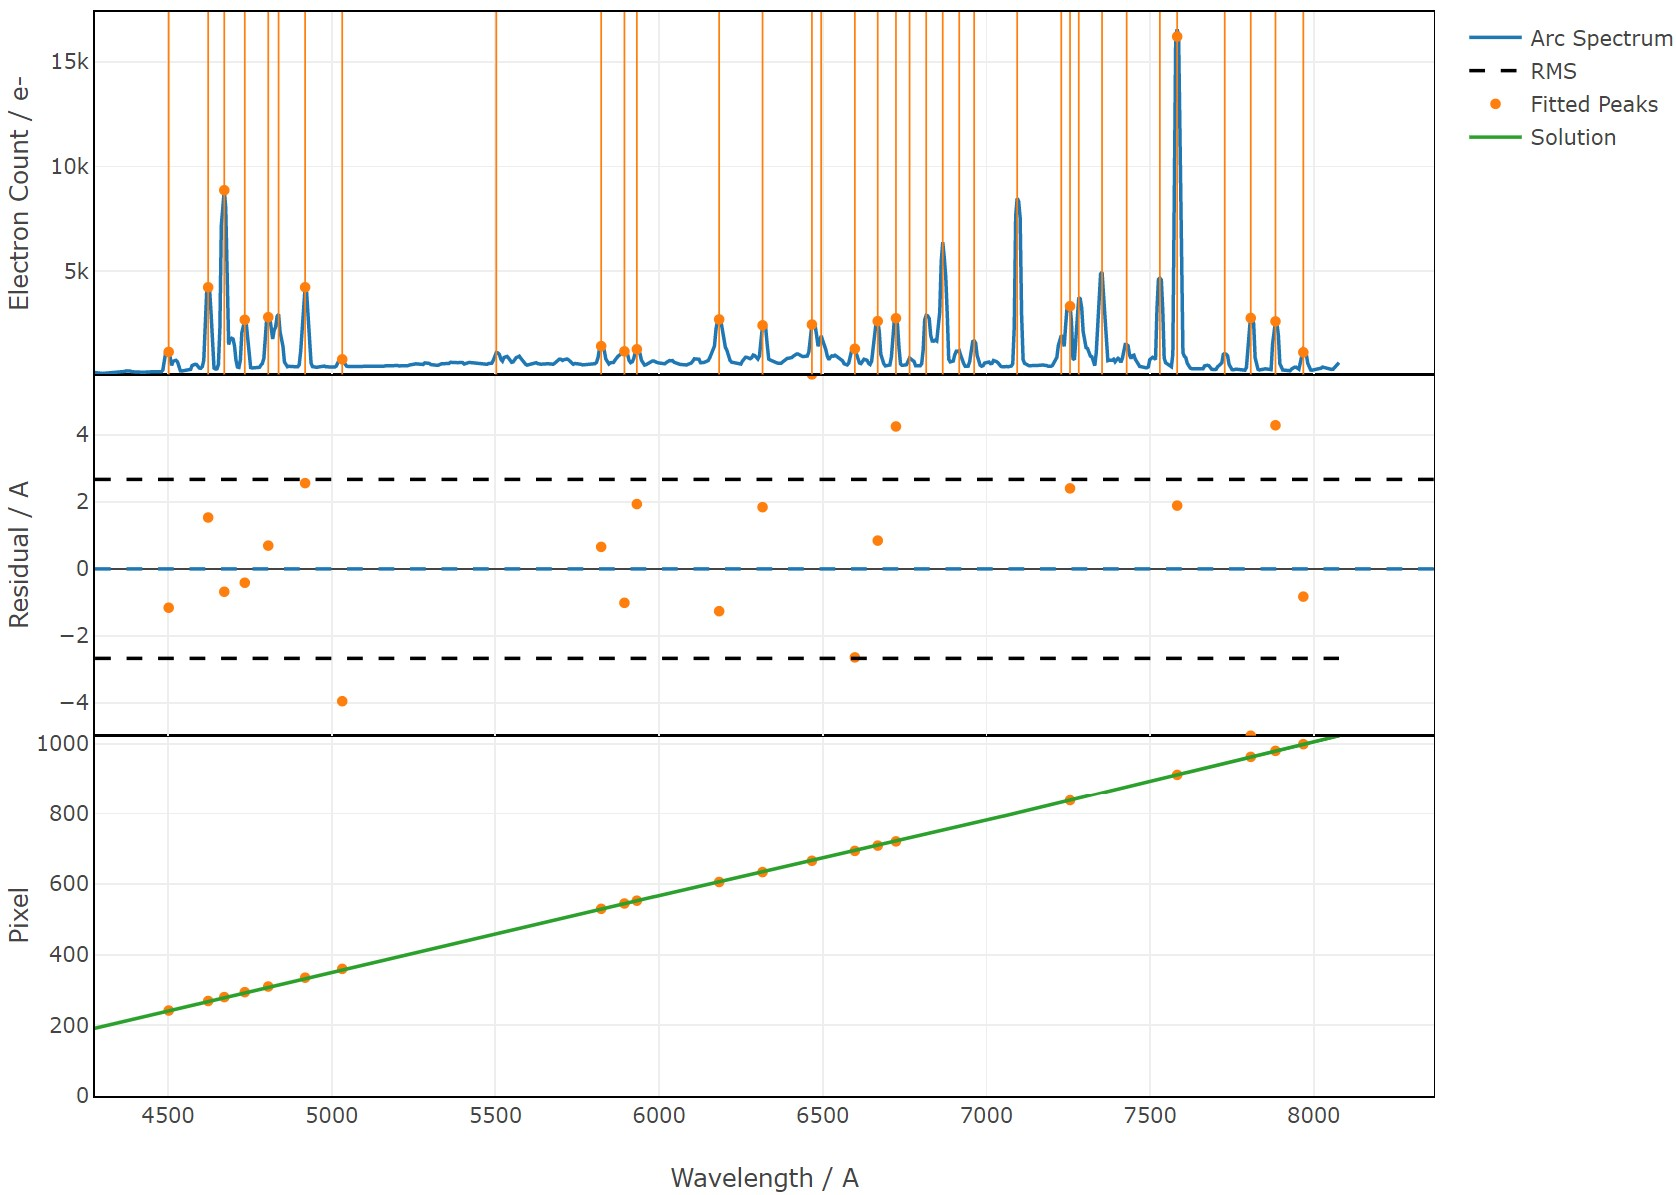
\includegraphics[width=\columnwidth]{fig_05_wavelength_calibration_diagnostics.jpg}
    \caption{Caption}
    \label{fig:wavecal}
\end{figure}

\subsection{Flux Calibration}
When a standard spectrum is wavelength calibrated, it can be
compared against the literature values to obtain the sensitive
function of the detector. All the standard stars available in
\textsc{iraf}\footnote{\url{https://github.com/iraf-community/iraf/tree/main/noao/lib/onedstds}}
and on the ESO webpage -- \textit{Optical and UV Spectrophotometric
Standard Stars}\footnote{\url{https://www.eso.org/sci/observing/tools/standards/spectra.html}}.
See also the Appendix for the complete listing of the standard
stars and the respective spectral ranges.
The calibration can be done in either AB magnitude or in
flux density~(per unit wavelength). The two should give similar
results but the response functions found would not be equivalent
because fitting with the magnitudes is a fit in the logarithmic
space compared to that in flux density, smoothing~(see below)
will have different effect in the two spaces.

\subsubsection*{Smoothing}
A Savitzky-Golay smoothing
filter\footnote{\url{https://docs.scipy.org/doc/scipy/reference/generated/scipy.signal.savgol_filter.html}}~\citep[hereafter, SG-filter]{1964AnaCh..36.1627S}
can be applied to the data before computing the sensitivity curve.
This function works by fitting low-order polynomials to localised
subsets of the data to suppress noise in the data as each point
interval. It is similar to the commonly used median boxcar filter,
but this uses more weighted information that allows better
retention of information while removing noise. This can be
used independent or in conjunction with the continuum fitting which
uses a LOWESS filter. By default, the SG-filter is only removing
significant noise~(e.g.\ those from cosmic rays).

\subsubsection*{Continuum Fitting}
By default, the continuum of the standard spectrum is found for
deriving the sensitivity curve. This process is used after the
smoothing procedure if that is set to True. The continuum is found
by fitting the standard spectrum with the same LOWESS function
used in fitting the line-spread-function as described in
Sec.~\ref{sec:extract}. This removes the random noise and avoid
fitting over the absorption bands (e.g.\ broad Balmer lines in
white dwarf standards) when computing the sensitivity.

\subsection*{Sensitivity Curve}
The sensitivity curve is computed by dividing the observed standard
spectrum by the literature one. This can be done without any smoothing
or directly with continuum fitting, or with either or both of them.
An interpolated spline or a polynomial can be computed as the
sensitivity curve. Users can manually supply a response function in
the format as a callable function (accept wavelength value and returning the
sensitivity value). It does not carry the concept of unit in the y-axis,
it can be in magnitude, flux, or any other appropriate unit for the
reduction.

\subsubsection*{Atmospheric Extinction Correction}
\textsc{ASPIRED} has a built-in atmospheric extinction curve based on
the Technical Note No. 31 \textit{Atmospheric extinction at the Roque
de Los Muchachos observatory, La Palma} of the Isaac Newton Group of
Telescopes~\footnote{\url{http://www.ing.iac.es/astronomy/observing/manuals/man_tn.html}}.
It reports the extinction in the unit of magnitude per airmass as a
function of wavelength between 3000 and 10000\AA. Alternatively,
a callable function in the appropriate units can be supplied to
perform the extinction correction.

\section{Deployment}

%\subsection{Liverpool Telescope/SPRAT}

%\subsection{Leseide Telescope/MOKOODI}

\section{Distribution}
The \textsc{ASPIRED} is released under the BSD (3-Clause) License. The
source code is hosted on \textsc{Github}, which can be found at
\verb+https://github.com/cylammarco/ASPIRED+, the tagged copied together
with the DOI of each version can be found at
\textsc{zenodo} \verb+https://zenodo.org/record/4463569#.YLjdrKgzYrQ+.
For simpler installation process, they are also available at Python
Package Index~(PyPI): \verb+https://pypi.org/project/aspired/+ such that
users can install the software by a simple command of 
\begin{verbatim}
    pip install aspired.
\end{verbatim}
In the future, we intend to expand this to allow installation from
\textsc{conda}.

\section*{Acknowledgements}
This work was partially supported by OPTICON. This project has
received funding from the European Union’s Horizon 2020 research and
innovation programme under grant agreement No 730890. This material
reflects only the authors views and the Commission is not liable for
any use that may be made of the information contained therein.

This work was partially supported by the Polish NCN grant Daina
No. 2017/27/L/ST9/03221.

(Iair's ERC)

The LT is operated on the island of La Palma by Liverpool
John Moores University in the Spanish Observatorio del Roque
de los Muchachos of the Instituto de Astrof{\'i}sica de Canarias with
financial support from the UK Science and Technology Facilities
Council.

This work makes use of observations from the Las Cumbres Observatory
global telescope network. We have made use of the data collected from
the FLOYDS spectrograph on the LCOGT 2m telescope at both Siding Spring,
Australia and Maui, HI, United States.

%%%%%%%%%%%%%%%%%%%% REFERENCES %%%%%%%%%%%%%%%%%%

% The best way to enter references is to use BibTeX:

\bibliographystyle{mnras}
\bibliography{main} % if your bibtex file is called example.bib

%%%%%%%%%%%%%%%%%%%%%%%%%%%%%%%%%%%%%%%%%%%%%%%%%%

%%%%%%%%%%%%%%%%% APPENDICES %%%%%%%%%%%%%%%%%%%%%

\appendix

\section{Standard Stars}

%%%%%%%%%%%%%%%%%%%%%%%%%%%%%%%%%%%%%%%%%%%%%%%%%%


% Don't change these lines
\bsp	% typesetting comment
\label{lastpage}
\end{document}

% End of mnras_template.tex
